% introduction-to-programming-michaelmas-2010-summative.tex -- Summative report
%
% This is a solution of the summative assignment of the Introduction to
% Networks submodule of the Introduction to Programming module held at the
% Durham University, Durham, United Kingdom.  Michælmas term 2010.
%
% Based on \cite{minar}
%
% Copyright © 2008–2010 Jan Minář <rdancer@rdancer.org>
%
% This work is free software; you can redistribute it and/or modify
% it under the terms of the GNU General Public License version 2 (two),
% as published by the Free Software Foundation.
%
% This work is distributed in the hope that it will be useful,
% but WITHOUT ANY WARRANTY; without even the implied warranty of
% MERCHANTABILITY or FITNESS FOR A PARTICULAR PURPOSE.  See the
% GNU General Public License for more details.
%
% You should have received a copy of the GNU General Public License along
% with this work; if not, write to the Free Software Foundation, Inc.,
% 51 Franklin Street, Fifth Floor, Boston, MA 02110-1301 USA.

\documentclass[10pt]{report}


\usepackage[utf8]{inputenc}
\pdfoutput=1
\usepackage[pdftex]{graphicx}     
\usepackage{amssymb}    
\usepackage{harvard}
\usepackage{url}
\usepackage{fancyhdr}
\usepackage{lastpage}

\pagestyle{fancy}
\fancyhead{}
%\chead{Introduction to Programming --- Summative Assignment}
%\chead{Copyright © 2008–2010 Jan Minář {\tt <rdancer@rdancer.org>}}
	%\\ page \thepage\ of \pageref{LastPage}}

\chead{
    Introduction to Programming --- Summative Assignment\\
    Copyright © 2008–2010 Jan Minář {\tt <rdancer@rdancer.org>}
}

\author{Jan Minář {\tt <rdancer@rdancer.org>}}
%\date{November 28, 2008}

%%%%%%%%%%%%%%%%%%%%%%%%%%%%%%%%%%%%%%%%%%%%%%%%%%%%%%%%%%%%%%%%%%%%%%%%%%%%%%
% ``Title''
%	-- the assignment

% No LaTeX command to make a subtitle, but possible using custom code (not
% including due to absence of license, but it is possible):
% <http://groups.google.com/group/comp.text.tex/msg/3aa4f67d8b3a979b?hl=en-EN&pli=1>
\title{Introduction to Programming\\Summative Assignment}

\begin{document}
\bibliographystyle{agsm}

\maketitle

% Note: This is a ‘report’


%%%%%%%%%%%%%%%%%%%%%%%%%%%%%%%%%%%%%%%%%%%%%%%%%%%%%%%%%%%%%%%%%%%%%%%%%%%%%%
% ``Abstract (10%) Brief (about 100 words) summary of the main points. Write
% this last.''
%	-- the assignment
\chapter{Abstract}
\thispagestyle{fancy}
This work is in part based on \cite{minar}

%%%%%%%%%%%%%%%%%%%%%%%%%%%%%%%%%%%%%%%%%%%%%%%%%%%%%%%%%%%%%%%%%%%%%%%%%%%%%%
% ``Introduction (20%) Explain the hypothesis(es) of the experiment so an
% informed reader can understand why you are doing what you are doing.''
%	-- the assignment
\chapter{Introduction}
\thispagestyle{fancy}

%%%%%%%%%%%%%%%%%%%%%%%%%%%%%%%%%%%%%%%%%%%%%%%%%%%%%%%%%%%%%%%%%%%%%%%%%%%%%%
% ``Method (20%) What did you did, in enough detail that somebody else could
% replicate the experiment if they so wished. Feel free to adapt my
% instructions. Make explicit any assumptions or limitations of the method.''
%	-- the assignment
\chapter{Method}
\thispagestyle{fancy}

%%%%%%%%%%%%%%%%%%%%%%%%%%%%%%%%%%%%%%%%%%%%%%%%%%%%%%%%%%%%%%%%%%%%%%%%%%%%%%
% ``Results (20%) Present your results numerically, using tables, graphs,
% charts, summary statistics (e.g. averages) as appropriate.''
%	-- the assignment
\chapter{Results}
\thispagestyle{fancy}

%%%%%%%%%%%%%%%%%%%%%%%%%%%%%%%%%%%%%%%%%%%%%%%%%%%%%%%%%%%%%%%%%%%%%%%%%%%%%%
% ``Discussion (20%) What do your results have to say about the hypotheses?''
%	-- the assignment
\chapter{Discussion}
\thispagestyle{fancy}

%%%%%%%% \chapter{Client-Server Architecture}
%%%%%%%% \thispagestyle{fancy}
%%%%%%%% 
%%%%%%%% In a client-server architecture, the application is distributed over two or
%%%%%%%% more separate platforms.  The servers offer services which are utilized by the
%%%%%%%% clients.  One functional unit can act both as a client and a server at the same time
%%%%%%%% (e.g.\ a web server that is at the same time a client to a database server).
%%%%%%%% Clients and servers communicate over shared network. \cite[pp3--11]{vaughn}
%%%%%%%% 
%%%%%%%% There is a vast number of applications that follow the client-server model
%%%%%%%% (most of the ports assigned by IANA correspond to client-server applications
%%%%%%%% \cite{iana}).  Alternatives to the client-server architecture include
%%%%%%%% {\em application} architecture and {\em peer-to-peer} architecture.  \cite[p110]{kurose}
%%%%%%%% 
%%%%%%%% There is typically one or a few servers, serving a large number of clients
%%%%%%%% \cite[p110]{kurose}.  It is not possible for clients to communicate
%%%%%%%% with each other directly; all communication between clients must be
%%%%%%%% realized through the server (for example, two Mail User Agents 
%%%%%%%% can indeed send e-mails to each other, but always via e.g.\ SMTP and IMAP mail servers).
%%%%%%%% 
%%%%%%%% Maintaining a server can be ``infrastructure-intensive'', when the server has
%%%%%%%% to withstand very many requests.  Often a server farm is deployed, so that the
%%%%%%%% load is shared between multiple machines.  \cite[p110]{kurose}
%%%%%%%% 
%%%%%%%% \section{Transport Layer View}
%%%%%%%% 
%%%%%%%% The client initiates the communication by sending a request to the
%%%%%%%% server.  The server only {\em responds}, and can never {\em initiate}
%%%%%%%% communication.  If the initial request is to succeed, the server process
%%%%%%%% must have had requested the operating system to listen on a given (TCP
%%%%%%%% or UDP) port.  The port numbers and their corresponding services are
%%%%%%%% maintained by a central registry \cite{iana}, so that for example a POP3
%%%%%%%% client will be able to connect to a POP3 server just by knowing the
%%%%%%%% server IP address.  The port number only has to be specified when it differs
%%%%%%%% from the default.  Once the client sends in a request to the correct port and
%%%%%%%% address, request is received by the operating system of the server machine, the
%%%%%%%% operating system passes the request on to the server process.  The server
%%%%%%%% process responds to the request, and two-way communication ensues.
%%%%%%%% 
%%%%%%%% % % % % % % % % % % % % % % % % % % % % % % % % % % % % % % % % % % % % % % %
%%%%%%%% 
%%%%%%%% \section{Thick and Thin Clients}
%%%%%%%% 
%%%%%%%% A thin client system does most of the data processing on the server side.  This
%%%%%%%% allows the client to be relatively low-powered, which can mean lower costs
%%%%%%%% (network terminals used instead of full-blown PCs, with the applications running
%%%%%%%% on an application server), or perhaps longer battery life (mobile phone or a PDA
%%%%%%%% running a video-processing application client, with the actual computationally
%%%%%%%% intensive video re-encoding performed on the server accessed over the mobile network).  Early web browsers were thin clients.
%%%%%%%% 
%%%%%%%% A thick client does most of the data processing itself.  This approach
%%%%%%%% does not suffer from the limitations of the network, such as latency.
%%%%%%%% For example, high quality video playback is a bandwidth-intensive
%%%%%%%% application, and it is often more practical to transport the video over
%%%%%%%% the network in a compressed form, and have the client do the
%%%%%%%% computationally intensive decompression, thus saving bandwidth.
%%%%%%%% Contemporary web browsers are thick clients.
%%%%%%%% 
%%%%%%%% %%%%%%%%%%%%%%%%%%%%%%%%%%%%%%%%%%%%%%%%%%%%%%%%%%%%%%%%%%%%%%%%%%%%%%%%%%%%%%
%%%%%%%% 
%%%%%%%% %%%%%%%%%%%%%%%%%%%%%%%%%%%%%%%%%%%%%%%%%%%%%%%%%%%%%%%%%%%%%%%%%%%%%%%%%%%%%%
%%%%%%%% % ``There are TWO types of packet switching networks: virtual circuit and
%%%%%%%% % datagram.  Describe in detail the key features of each type?''
%%%%%%%% %	-- the assignment
%%%%%%%% 
%%%%%%%% \chapter{Key Features of Virtual Circuit and Datagram Packet Switching Networks}
%%%%%%%% \thispagestyle{fancy}
%%%%%%%% 
%%%%%%%% % Intro
%%%%%%%% 
%%%%%%%% {\em Virtual circuit} (VC; also called {\em virtual call}) networks came from the
%%%%%%%% traditional pre-existing voice telephone network, which was usually a state-wide
%%%%%%%% network, with interstate and overseas links.  The word ``datagram'' itself
%%%%%%%% derives from ``telegram'' \cite[p141]{russell}.  On the other hand, {\em packet
%%%%%%%% switching} was developed in the 1970s as means of efficient transmission of data
%%%%%%%% over long distances.  Nowadays, datagram networking takes over traditional mainstays of VC,
%%%%%%%% however, VC is still being used.  It is possible to use a mixed approach.
%%%%%%%% 
%%%%%%%% \section{Virtual Circuit Lifetime}
%%%%%%%% 
%%%%%%%% Connection via VC has three phases:
%%%%%%%% 
%%%%%%%% \begin{enumerate}
%%%%%%%% \item set-up
%%%%%%%%     \begin{itemize}
%%%%%%%%     %\item LCI (Logical Channel Identifier; the name of the single connection to the next node) is chosen
%%%%%%%%     \item the path through the network is determined
%%%%%%%%     \item resources such as bandwidth/time slot are reserved, and everything is set
%%%%%%%%     \item this can take some amount of time, creating a set-up delay
%%%%%%%%     \end{itemize}
%%%%%%%% \item data transfer
%%%%%%%%     \begin{itemize}
%%%%%%%%     %\item nodes use LCI
%%%%%%%%     \item the path does not changed for the duration of the connection
%%%%%%%%     \item resources remain reserved even when not actually needed
%%%%%%%%     \item the latency is negligible, because there are no delays introduced by the management of the link, unlike with datagram networks
%%%%%%%%     \end{itemize}
%%%%%%%% \item tear-down
%%%%%%%%     \begin{itemize}
%%%%%%%%         %\item the resources are freed
%%%%%%%% 	%\item LCI is forgotten
%%%%%%%% 	\item the routing table entries are purged
%%%%%%%% 	\item bandwidth/slots are released for use for future VCs
%%%%%%%%     \end{itemize}
%%%%%%%% \end{enumerate}
%%%%%%%% 
%%%%%%%% \section{Routing in Datagram Networks}
%%%%%%%% 
%%%%%%%% Datagram networks route each packet individually.
%%%%%%%% When a datagram router receives a packet, it needs to decide which next
%%%%%%%% hop it should send it to, i.e.\ which interface to forward it via.  It
%%%%%%%% would be impractical to store this information for every possible
%%%%%%%% destination address, and therefore the routers mostly store only
%%%%%%%% aggregate routes (multiple adjacent addresses represented by a common
%%%%%%%% prefix).  Often an address is
%%%%%%%% comprised of a prefix, and a host part.  The routes are then
%%%%%%%% decided with respect to the network prefixes, not the individual
%%%%%%%% addresses.  A router can maintain two different routes for two network
%%%%%%%% prefixes in such a way that one prefix is contained in the other one.
%%%%%%%% In that case, the longer prefix takes precedence.  It is said that the
%%%%%%%% corresponding route is more specific.
%%%%%%%% 
%%%%%%%% As using hard-coded, or static routing would not be feasible for busy
%%%%%%%% routers with many connections, automatic routing protocols have been
%%%%%%%% devised that change routing table typically every few minutes.  In
%%%%%%%% contrast to that, in a VC network, the routing table constantly changes
%%%%%%%% with every VC setup/tear-down, many times a second.
%%%%%%%% 
%%%%%%%% 
%%%%%%%% %\section{History}
%%%%%%%% %
%%%%%%%% %In telephony systems, complexity is kept within the network, which allows
%%%%%%%% %``dumb'' end-systems as simple as rotary phones be connected.  Internet was on
%%%%%%%% %the other hand designed to connect sophisticated hosts, and designed
%%%%%%%% %deliberately to be ``as simple as possible''.  Complex functionality is
%%%%%%%% %implemented by the {\em transport} and {\em application} layers.  The internet
%%%%%%%% %{\em network} layer is easy to implement over disparate range of {\em link} layer
%%%%%%%% %technologies, such as ``satellite, Ethernet, fiber, or radio''.  It's also easy
%%%%%%%% %to implement new applications, because all that is required is to implement them
%%%%%%%% %in the end hosts; changes to the network are not necessary.
%%%%%%%% %\cite[pp349--351]{kurose}
%%%%%%%% 
%%%%%%%% \section{Comparison}
%%%%%%%% 
%%%%%%%% \begin{table}[h]
%%%%%%%%   \begin{tabular}{ | p{6cm} | p{6cm} | }
%%%%%%%%   \hline
%%%%%%%% 
%%%%%%%%   {\em Virtual Circuit}
%%%%%%%%   	& {\em Datagram} \\ \hline
%%%%%%%%   \hline
%%%%%%%% 
%%%%%%%% complexity is kept within the network, which allows end-systems to be simple,
%%%%%%%% even ``dumb'' \cite[p349]{kurose}
%%%%%%%% 	& designed to connect sophisticated
%%%%%%%% 	hosts, the network is deliberately ``as simple as possible'';  complex functionality is implemented by the {\em transport} and {\em application} layers \cite[pp349--351]{kurose}
%%%%%%%% 	\\ \hline
%%%%%%%% 
%%%%%%%% maintains a dedicated path through the network between the two end-hosts 
%%%%%%%% 	& routes each packet separately, each packet contains routing
%%%%%%%% 	information header; path can change in-between packets \\ \hline
%%%%%%%% 
%%%%%%%% guarantees delivery, low latency and reserved bandwidth
%%%%%%%% 	& best-effort, with packet loss/duplicity, jitter, data corruption,
%%%%%%%% 	shared bandwidth \\ \hline
%%%%%%%% 
%%%%%%%% its all-or-nothing approach means it will simply fail hard and tear down the
%%%%%%%% connection in case of an error
%%%%%%%% 	&  routes around a malfunctioning router or network path and recovers
%%%%%%%% 	from errors \\ \hline
%%%%%%%% 
%%%%%%%% naturally maps onto traditional voice networks, which it was developed from and
%%%%%%%% for
%%%%%%%% 	& developed in the 1970s; has not fundamentally changed since, one
%%%%%%%% 	of few technologies of choice for data transmission over long distances
%%%%%%%% 	\cite[p298--299]{stallings} \\ \hline
%%%%%%%% 
%%%%%%%% good for voice, video \& similar real-time, low-latency applications that
%%%%%%%% require approximately the same amount of bandwidth all the time
%%%%%%%% 	& good for applications that transmit data in bursts \\ \hline
%%%%%%%% 
%%%%%%%% upfront delay while the virtual circuit is set up; latency negligible afterwards
%%%%%%%% 	& considerable latency due to intrinsic delays \\ \hline
%%%%%%%% 
%%%%%%%%   \end{tabular}
%%%%%%%%   \caption{Comparison of Virtual Circuit and Datagram Networks}
%%%%%%%%   \label{vcdgcomparison}
%%%%%%%% \end{table} 
%%%%%%%% 
%%%%%%%% 
%%%%%%%% Table \ref{vcdgcomparison} compiled from data in \cite{kurose,russell},
%%%%%%%% \cite[p298--299]{stallings}.
%%%%%%%% 
%%%%%%%% %Some see it as an advantage that instead of using the (long) address, only the
%%%%%%%% %(short) Logical Channel Identifier (LCI) is used.  This will save bandwidth,
%%%%%%%% %complexity and processing power, compared to having to compute the route for
%%%%%%%% %every datagram. \cite[p158]{russell} (the addresses are only used/needed during
%%%%%%%% %the initial phase of connection set-up).  However, there are ways to approximate
%%%%%%%% %these advantages even in datagram networks.
%%%%%%%% %
%%%%%%%% %Virtues of the VC technology do not prevent errors in other parts of
%%%%%%%% %the application.  Properly engineered system will function correctly
%%%%%%%% %regardless of which of the two approaches is used \cite[p161]{russell}
%%%%%%%% %
%%%%%%%% %Some applications can not take advantage of the VC guaranteed
%%%%%%%% %sequentiality \cite[p161]{russell}
%%%%%%%% %
%%%%%%%% %The VC advantage of link and CPU efficiency due to using the LCI in
%%%%%%%% %place of the full address is not so marked when workarounds and
%%%%%%%% %real-life costs are taken into account: datagram network does not have
%%%%%%%% %to work with the full-length representation of an address, and replacing
%%%%%%%% %the (long) address with a (short) LCI does not necessarily prove to
%%%%%%%% %result in significant savings \cite[p161]{russell}
%%%%%%%% 
%%%%%%%% \section{Hybrid Approach}
%%%%%%%% 
%%%%%%%% ``[V]irtual circuit can be built on top of the datagram service''
%%%%%%%% \cite[p141]{russell}.  Many currently deployed networks behave like a VC towards the end-hosts,
%%%%%%%% and are really internally working as datagram networks---the advantage
%%%%%%%% of having a comfortable interface presented to the host is married with
%%%%%%%% the flexibility and cost-efficiency of a datagram network.
%%%%%%%% %%%%%%%%%%%%%%%%%%%%%%%%%%%%%%%%%%%%%%%%%%%%%%%%%%%%%%%%%%%%%%%%%%%%%%%%%%%%%%
%%%%%%%% 
%%%%%%%% 
%%%%%%%% 
%%%%%%%% %%%%%%%%%%%%%%%%%%%%%%%%%%%%%%%%%%%%%%%%%%%%%%%%%%%%%%%%%%%%%%%%%%%%%%%%%%%%%%
%%%%%%%% % ``There are a wide range of application layer protocols including the
%%%%%%%% % Hypertext Transfer Protocol (HTTP).  Describe HTTP in detail and be sure to
%%%%%%%% % include in your description HTTP's function (what does it do), design (why
%%%%%%%% % does it do it), and behaviour (how does it do it).''
%%%%%%%% %	-- the assignment
%%%%%%%% 
%%%%%%%% \chapter{Hypertext Transfer Protocol}
%%%%%%%% \thispagestyle{fancy}
%%%%%%%% %%%%%%%%%%%%%%%%%%%%%%%%%%%%%%%%%%%%%%%%%%%%%%%%%%%%%%%%%%%%%%%%%%%%%%%%%%%%%%
%%%%%%%% 
%%%%%%%% The Hypertext Transfer Protocol is a public domain client-server
%%%%%%%% stateless application layer protocol that communicates over TCP.
%%%%%%%% \cite{rfc1945,rfc2616},
%%%%%%%% \cite[pp122--124]{kurose}
%%%%%%%% 
%%%%%%%% HTTP is the most often used data transport application protocol on the
%%%%%%%% World Wide Web.
%%%%%%%% 
%%%%%%%% \section{Function}
%%%%%%%% 
%%%%%%%% HTTP retrieves and manipulates objects denoted by Uniform Resource Identifiers
%%%%%%%% (URIs).  \cite{stallings} HTTP methods GET, PUT, DELETE, MOVE, LINK, UNLINK are
%%%%%%%% used for this purpose.  HTTP has auxiliary capabilities represented by the
%%%%%%%% methods HEAD OPTIONS, TRACE, CONNECT and others.
%%%%%%%% 
%%%%%%%% HTTP has built-in support for caches.  Cache is an intermediate web server that
%%%%%%%% takes the HTTP requests and if possible serves the objects from a local
%%%%%%%% repository, thereby providing speedier response and saving Internet bandwidth.
%%%%%%%% 
%%%%%%%% \section{Behaviour}
%%%%%%%% 
%%%%%%%% HTTP uses several powerful technologies, some of them predating its invention,
%%%%%%%% some of them invented because of HTTP.  Underlying character set is
%%%%%%%% human-readable ASCII.  Reliable transport is provided by TCP.  The protocol
%%%%%%%% leverages the very powerful concept of URIs/URLs \cite{rfc1738} to identify the
%%%%%%%% objects that are to be manipulated.  HTTP also uses MIME, and other technologies
%%%%%%%% to negotiate the presentation of the object identified by the URI.\cite{rfc2616}
%%%%%%%% HTTP then retrieves the object.
%%%%%%%% 
%%%%%%%% \section{Design}
%%%%%%%% 
%%%%%%%% HTTP was designed to transfer simple textual web pages on the World Wide Web
%%%%%%%% efficiently.  Because a typical web session has the user retrieving pages in a
%%%%%%%% quick succession from different servers, the protocol was designed to have low
%%%%%%%% overhead, and be stateless.  By the time HTTP 1.1 was designed, the Web changed
%%%%%%%% radically, and a need for multi-object web pages was felt, as well as usefulness
%%%%%%%% of tracking the user across visits.  Therefore, persistent connections and
%%%%%%%% pipelining was added, and HTTP cookies.  Other functionality, such as the
%%%%%%%% support for virtual servers (the Host header) has been added.
%%%%%%%% 
%%%%%%%% 
%%%%%%%% \section{Packet Dissection}
%%%%%%%% 
%%%%%%%% We have prepared two HTTP packets out of a TCP stream that was the
%%%%%%%% result of retrieving a single document from a remote WWW server.  The
%%%%%%%% upper half of the images shows the interpretation, the lower half then
%%%%%%%% the on-the-wire data in hexadecimal and ASCII representation.  We used
%%%%%%%% {\em Wireshark} 1.0.0 to perform the packet analysis.
%%%%%%%% 
%%%%%%%% \begin{figure}[p]
%%%%%%%%     \centering
%%%%%%%%     % Border around the image
%%%%%%%%     \setlength\fboxsep{0pt}
%%%%%%%%     \setlength\fboxrule{0.5pt}
%%%%%%%%     \fbox{
%%%%%%%% 	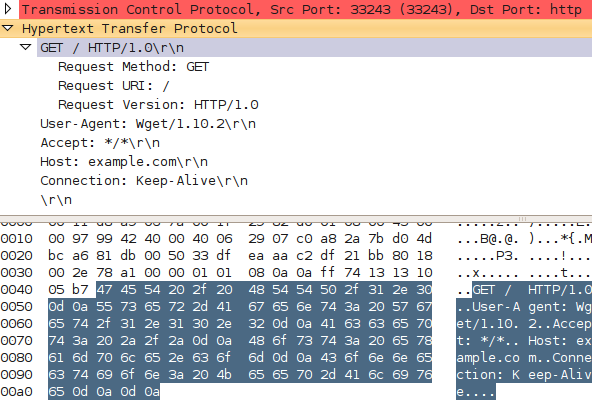
\includegraphics[width=0.8\textwidth]{http-get.png}
%%%%%%%%     }
%%%%%%%%     \caption{HTTP request}
%%%%%%%%     \label{httprequest}
%%%%%%%% \end{figure}
%%%%%%%% 
%%%%%%%% Figure \ref{httprequest} shows the HTTP request. 
%%%%%%%% TCP packet sent to HTTP default port (denoted by {\em http}; 80), the well-known port number assigned to HTTP.
%%%%%%%% The request line specifies the GET method, path /, the HTTP version used is 1.0.
%%%%%%%% The User Agent (UA) claims to be Wget version 1.10.2, and it accepts any and all MIME types.
%%%%%%%% URI host part is example.com.  The UA wishes to use persistent connections.
%%%%%%%% Entity body is empty.
%%%%%%%% 
%%%%%%%% \begin{figure}[p]
%%%%%%%%     \centering
%%%%%%%%     % Border around the image
%%%%%%%%     \setlength\fboxsep{0pt}
%%%%%%%%     \setlength\fboxrule{0.5pt}
%%%%%%%%     \fbox{
%%%%%%%% 	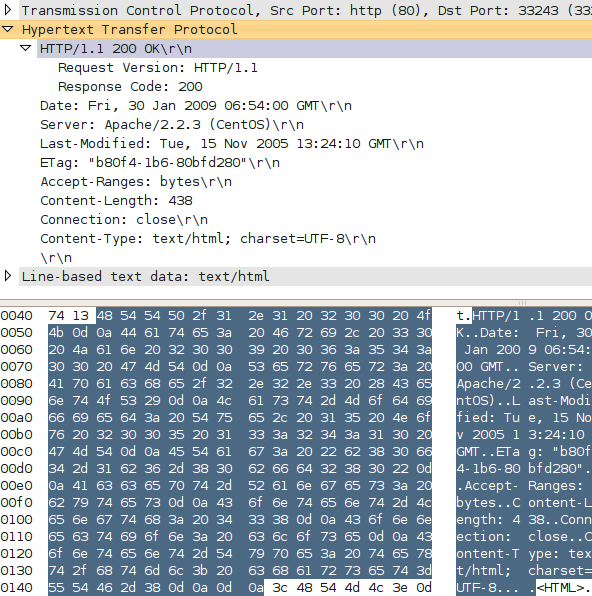
\includegraphics[width=0.8\textwidth]{http-200-ok.png}
%%%%%%%%     }
%%%%%%%%     \caption{HTTP response}
%%%%%%%%     \label{httpresponse}
%%%%%%%% \end{figure}
%%%%%%%% 
%%%%%%%% Figure \ref{httpresponse} shows the HTTP response.
%%%%%%%% The status line shows the server uses HTTP version 1.1, status code 200 means
%%%%%%%% that the request has been successfully processed.  The response was generated on
%%%%%%%% 2009-01-30 at 06:54:00 GMT.  Server claims to be Apache version 2.2.3 running on
%%%%%%%% CentOS.  The requested object has not been modified since 2005-11-15 13:24:10
%%%%%%%% GMT.  The entity tag (ETag) is given.  Server accepts byte-range requests.
%%%%%%%% Length of the entity body is 438 octets.  Server will close the TCP connection
%%%%%%%% when the entity body will have been transmitted.  The MIME type of the object is
%%%%%%%% text/html, character set UTF-8.  The entity body contains the requested object
%%%%%%%% (the HTML page).
%%%%%%%% 
%%%%%%%% %%%%%%%%%%%%%%%%%%%%%%%%%%%%%%%%%%%%%%%%%%%%%%%%%%%%%%%%%%%%%%%%%%%%%%%%%%%%%%
%%%%%%%% % ``There are TWO types of transport layer service that the Internet provides
%%%%%%%% % to its applications, connection-oriented services and connectionless
%%%%%%%% % services.
%%%%%%%% % ``a) Describe in detail the characteristics of connection-oriented services.
%%%%%%%% % ``b) Describe in detail the characteristics of connectionless services.''
%%%%%%%% %	-- the assignment
%%%%%%%% 
%%%%%%%% \chapter{Characteristics of Connection-Oriented and Connectionless Transport
%%%%%%%% 	Layer Services}
%%%%%%%% \thispagestyle{fancy}
%%%%%%%% 
%%%%%%%% The two most prolific Internet Protocol Suite transport layer protocols are UDP
%%%%%%%% and TCP.  We will show the characteristics of connection-oriented and
%%%%%%%% connectionless services using UDP and TCP as examples and describing briefly how
%%%%%%%% they work.
%%%%%%%% 
%%%%%%%% \section{Connectionless Service---User Datagram Protocol}
%%%%%%%% 
%%%%%%%% UDP is defined in \cite{rfc768}.  It is the datagram transport in the
%%%%%%%% Internet Protocol Suite.  It is a very thin layer on top
%%%%%%%% of IP, as it only provides a checksum and port number (enabling
%%%%%%%% multiplexing, i.e.\ having more than one connection from one host to
%%%%%%%% another via UDP). (Cf.\ Fig.\ \ref{udpheader}) \cite{rfc1180}
%%%%%%%% 
%%%%%%%% \begin{figure}[h]
%%%%%%%%     \label{udpheader}
%%%%%%%%     \centering
%%%%%%%%     % Border around the image
%%%%%%%% 	\begin{verbatim}
%%%%%%%%               0      7 8     15 16    23 24    31  
%%%%%%%%               +--------+--------+--------+--------+
%%%%%%%%               |     Source      |   Destination   |
%%%%%%%%               |      Port       |      Port       |
%%%%%%%%               +--------+--------+--------+--------+
%%%%%%%%               |                 |                 |
%%%%%%%%               |     Length      |    Checksum     |
%%%%%%%%               +--------+--------+--------+--------+
%%%%%%%%               |                                    
%%%%%%%%               |          data octets ...           
%%%%%%%%               +---------------- ...                
%%%%%%%% 	\end{verbatim}
%%%%%%%%     \caption{User Datagram Protocol Header
%%%%%%%% 	    % XXX DNW
%%%%%%%% 	    %\cite{rfc768}
%%%%%%%% 	    (Postel 1980, p1) % Verbatim: DWIT!
%%%%%%%%     }
%%%%%%%% \end{figure}
%%%%%%%% 
%%%%%%%% The connectionless service only provides the bare minimum necessary for
%%%%%%%% a transport layer to provide.  This can be a positive feature, because
%%%%%%%% it means low overhead and low implementation complexity.
%%%%%%%% 
%%%%%%%% UDP provides the application layer with the ability to send and receive short
%%%%%%%% fixed-length datagrams.   Each datagram is a separate transmission; there is no
%%%%%%%% state kept in-between.  If desired, the application can implement some of the
%%%%%%%% missing features in a higher layer.
%%%%%%%% 
%%%%%%%% \section{Connection-Oriented Service---Transport Control Protocol}
%%%%%%%% 
%%%%%%%% TCP \cite{rfc793} is the most commonly used transport protocol in the
%%%%%%%% Internet Protocol Suite.  In order to provide a connection-oriented service, the
%%%%%%%% protocol is necessarily more complex than its connectionless
%%%%%%%% counterpart.  The complexity comes at cost in bandwidth and processing
%%%%%%%% overhead.
%%%%%%%% 
%%%%%%%% TCP provides in-order reliable delivery (with automatic retransmission
%%%%%%%% of lost packets) and automatic congestion sensing and adaptation.  Like
%%%%%%%% UDP, TCP provides corruption checking using checksum, and multiplexing
%%%%%%%% using ports.  TCP provides the application layer with an abstraction of
%%%%%%%% a transparent end-to-end duplex virtual circuit (byte stream).
%%%%%%%% \cite{rfc1180}
%%%%%%%% 
%%%%%%%% %\subsection{How TCP Operates}
%%%%%%%% %
%%%%%%%% %Similarly to a link-layer Virtual Circuit, there are three phases of
%%%%%%%% %TCP operation:
%%%%%%%% %
%%%%%%%% %\begin{enumerate}
%%%%%%%% %    \item connection set-up
%%%%%%%% %    \item data transfer
%%%%%%%% %    \item connection tear-down
%%%%%%%% %\end{enumerate}
%%%%%%%% %
%%%%%%%% %Connection set-up is performed using a three-way handshake.  Once that
%%%%%%%% %is done, TCP accepts data from the application layer.  The connection
%%%%%%%% %comes to an end when either host terminates the connection, or the
%%%%%%%% %connection times out.
%%%%%%%% %
%%%%%%%% %Every successfully received packet is acknowledged.  Acknowledge
%%%%%%%% %packets can piggy-back on data packets sent to the other host.
%%%%%%%% %
%%%%%%%% %TCP uses a {\em sliding window} to determine whether a given packet has
%%%%%%%% %been received.  At any given time, as many bytes as can fit in the
%%%%%%%% %window can remain unacknowledged.  When the number of bytes goes over
%%%%%%%% %the size of the window, the packet is presumed lost.  The size of the
%%%%%%%% %window changes during the transmission, to accommodate changes in
%%%%%%%% %link throughput, and congestion control.
%%%%%%%% %
%%%%%%%% %%%%%%%%%%%%%%%%%%%%%%%%%%%%%%%%%%%%%%%%%%%%%%%%%%%%%%%%%%%%%%%%%%%%%%%%%%%%%%



%
% References
%

%%%%%%%%%%%%%%%%%%%%%%%%%%%%%%%%%%%%%%%%%%%%%%%%%%%%%%%%%%%%%%%%%%%%%%%%%%%%%%
% ``References and presentation (10%) Take care to refer to any source
% material appropriately, using an appropriate citation style (Coxhead 2009 "A
% Referencing Style Guide", http://www.cs.bham.ac.uk/~pxc/refs/refs.html
% [accessed 18 Nov 2010]). The mark of 10% includes appropriate referencing
% and appropriate presentation throughout the document.''
%	-- the assignment

\bibliography{references,rfc}
\thispagestyle{fancy}

\end{document}
